\chapter[Идентификация нелинейных стохастических систем второго типа]{%
  Идентификация нелинейных стохастических систем второго типа
}

\section{Математическая модель идентифицируемой системы}

Для обеспечения наглядности сравнения рассматривался случай идентификации скалярной системы:
\begin{equation}
  \label{eq:nonlinear_model_scalar}
  \begin{aligned}
  h &= \psi(\overline{\theta}, \xi), \\
  x &= \xi + \varepsilon_x, \\
  y &= h + \varepsilon_y,
  \end{aligned}
\end{equation}
где \( \xi, h \) "--- фактические значения входной и выходной переменной, \par
\( \psi \) "--- скалярно-векторная функция регрессии, \par
\(
\overline{\theta} = (\theta_1, \theta_2, \dotsc, \theta_m)
\) "--- вектор фактических значений параметров объекта, \par
\( x, y \) "--- измеренные значения входной и выходной переменной, \par
\( \varepsilon_x, \varepsilon_y \) "--- независимые ошибки измерений значений входной и
выходной переменной, распределенные по нормальному закону:
\(
\varepsilon_x = N(0, \sigma_{\varepsilon_x}),
\varepsilon_y = N(0, \sigma_{\varepsilon_y})
\).

\section{Алгоритмы методов идентификации}

\subsection{Нелинейный метод наименьших квадратов}

Один из подходов к оценке параметров системы~\eqref{eq:nonlinear_model_scalar} состоит в следующем.
Можно <<закрыть глаза>> на существование ошибок измерений
входной переменной, то есть считать, что \( \varepsilon_x = 0 \),
и вместо данной модели рассматривать модель
\begin{equation}
  \label{eq:nonlinear_model_lse}
  \begin{aligned}
  x &= \psi(\overline{\theta}, \xi), \\
  y &= x + \varepsilon_y.
  \end{aligned}
\end{equation}

Тогда оценка вектора параметров объекта определяется выражением~\cite{mukha_2009}
\begin{equation}
  \label{eq:nonlinear_lse}
  \hat{\overline{\theta}}_{\text{НМНК}} =
  \overline{\theta}_0 + (Q^T R^{-1}_{\Xi} Q)^{-1} Q^T R^{-1}_{\Xi} (y - \psi(\overline{\theta}_0, x)),
\end{equation}
где \( \overline{\theta}_0 \) --- опорная точка,
\( Q = \dfrac{\partial \psi(\overline{\theta}_0, x) }{ \partial \overline{\theta}_0 } \).

Эту оценку будем называть оценкой, полученной нелинейным
методом наименьших квадратов (НМНК-оценкой).
В качестве опорной точки \( \overline{\theta}_0 \) можно использовать значения
\( \theta_1, \dotsc, \theta_m \),
полученные в результате численного решения системы уравнений
\begin{equation}
  \label{eq:nonlinear_basic}
  (y_j - \psi( \overline{\theta}, x_j )) = 0, \: j = \overline{1,m},
\end{equation}
где \( x_j, y_j \) --- опорные наблюдения входа и выхода системы соответственно.

В качестве опорных значений могут выступать, например:
\begin{itemize}
\item первые \( m \) порядковых статистик из множества наблюдений:
  \[
    (x_1, y_1), (x_2, y_2), \dotsc , (x_m, y_m), \:
    x_i < x_{i+1}, \;
    i = \overline{1, n};
  \]
\item \( m \) равноотстоящих порядковых статистик:
  \[
    (x_{k}, y_{k}), (x_{2k}, y_{2k}) , \dotsc , (x_{mk}, y_{mk}), \:
    k = \lfloor \dfrac{n}{m} \rfloor, \:
    x_i < x_{i+1}, \;
    i = \overline{1, n};
  \]
\item \( m \) средних значений, рассчитанных на основе
  упорядоченного набора наблюдений:
  \begin{equation}
    \begin{gathered}
      ( \overline{x}_{k}, \overline{y}_{k} ),
      ( \overline{x}_{2k}, \overline{y}_{2k} ),
      \dotsc ,
      ( \overline{x}_{mk}, \overline{y}_{mk}), \\
      \overline{x}_{ik} = \dfrac{1}{m} \sum_{j = 1+(i-1)k}^{ik} x_j, \:
      \overline{y}_{ik} = \dfrac{1}{m} \sum_{j = 1+(i-1)k}^{ik} y_j, \\
      k = \lfloor \dfrac{n}{m} \rfloor \:
      x_i < x_{i+1}, \; i = \overline{1, n}.
    \end{gathered}
    \label{eq:nonlinear_base_values}
  \end{equation}
\end{itemize}

Для уточнения оценки, полученной по формуле~\eqref{eq:nonlinear_lse}, можно
организовать итерационную процедуру, заменяя опорную точку полученной оценкой.

\vspace{2\baselineskip}
\subsection{Метод рядов Тейлора}

Применение метода рядов Тейлора (МРТ) требует иной формулировки задачи,
допускаемой формулировкой \eqref{eq:nonlinear_model_scalar}.
Следует предположить, что \( j \)-е наблюдение вектора параметров \( \overline{\theta}_j \)
определяется как векторная функция показаний приборов:
\begin{equation}
  \label{eq:nonlinear_mrt_phi}
  \overline{\theta}_j = \phi( \overline{z}_{j} ), \: j = \overline{1, n},
\end{equation}
где вектор
\( \overline{z}^{\text{T}}_{j} =
( \overline{x}^{\text{T}}_{j}, \overline{y}^{\text{T}}_{j}) \)
имеет нормальное распределение \( N(A_{z,j}, R_{z,j}) \)
и оцениваемый векторный параметр \( \overline{\theta} \) определяется как
\( \overline{\theta} = \phi(A_{z,j}), \forall i = \overline{1, n} \).
В этом случае МРТ-оценка \( \hat{\overline{\theta}}_{\text{МРТ}} \) векторного параметра \( \overline{\theta} \)
определяется выражением
\begin{equation}
  \label{eq:nonlinear_mrt}
  \hat{\overline{\theta}}_{\text{МРТ}} =
  \Bigg( \sum^{n}_{i=1} R^{-1}_{\theta,i} \Bigg)^{-1}
  \sum^{n}_{j=1} R^{-1}_{\theta,j} \overline{\theta}_j,
\end{equation}
где
\( R_{\theta,i} = G_i R_{z,i} G^T_i \),
\( G_i =
\dfrac{\partial \phi( \overline{z}_{i} ) }{ \partial \overline{z}_{i} } \).

Численное значение наблюдения \( \theta_j \)~\eqref{eq:nonlinear_mrt_phi} может определяться как
решение системы уравнений~\eqref{eq:nonlinear_basic}.


\section{Численный анализ точности оценивания параметров}

\subsection{Методика сравнения}\label{subsec:nonlinear_comparison_conditions}

Было выполнено сравнение точности оценок,
полученных нелинейным методом наименьших квадратов и методом рядов Тейлора,
для функций регрессии различного вида,
в зависимости от с.~к.~о ошибок измеряемых значений
\( \sigma_{\varepsilon_x}, \sigma_{\varepsilon_y} \).

В качестве величины, характеризующей сравнительную точность оценивания параметров,
использовалась разность средних Евклидовых расстояний
между точными значениями параметров модели и их оценками, полученными
с помощью НМНК и МРТ:
\begin{equation}
  \begin{aligned}
    d &= d_{\text{НМНК}} - d_{\text{МРТ}}, \\
    d_{\text{НМНК}} &=
    \frac{1}{k} \sum_{j=1}^k
    \sqrt{\sum_{\text{i=1}}^m (\hat{\theta}_{\text{НМНК}_{ij}} - \theta_{ij})^2}, \\
    d_{\text{МРТ}} &=
    \frac{1}{k} \sum_{j=1}^k
    \sqrt{\sum_{\text{i=1}}^m (\hat{\theta}_{\text{МРТ}_{ij}} - \theta_{ij})^2}.
  \end{aligned}
  \label{eq:dst_nonlinear_param}
\end{equation}
Таким образом, при \( d > 0 \) точность оценивания параметров модели с помощью МРТ
превосходит точность НМНК, а при \( d < 0 \) НМНК-оценки являются более точными.
При \( d = 0 \) оба метода дают оценки одинаковой точности.

Значения \( \xi_i \) выбирались из равномерного в \( [0, 10] \) распределения.
Для получения каждой оценки \( \hat{\overline{\theta}} \) использовались результаты
ста наблюдений \( ( x_i, y_i ), i = \overline{1, n}, n = 100 \).

Расчеты величины \( d \) производились в узлах сетки значений
\( \sigma_{\varepsilon_x}, \sigma_{\varepsilon_y} \) в прямоугольнике
\( [0, 2] \times [0, 2] \) с шагом 0{,}1.
В каждом узле сетки вычислялось \( k = 100 \) оценок.
Для расчета оценок использовались опорные значения,
рассчитанные по алгоритму~\eqref{eq:nonlinear_base_values}.
В качестве значений НМНК-оценки \( \theta_{\text{НМНК}} \)
были использованы значения, полученные на первой итерации метода.

\pagebreak
\subsection{Линейная функция регрессии}

Простейшим частным случаем модели~\eqref{eq:nonlinear_model_scalar} является линейная,
то есть такая, функция регрессии которой имеет вид
\[ \psi = \theta_0 + \theta_1 \xi. \]

На рисунке~\ref{fig:comparison_nonlinear_linear}
представлен график зависимости \( d(\sigma_{\varepsilon_x}, \sigma_{\varepsilon_y}) \)
при \( \theta_1 = 1 \).
Видно, что точность оценок параметров модели, полученных с помощью НМНК,
превосходит точность МРТ-оценок.

По результатам исследования зависимости \( d \) при различных значениях
параметров модели можно сделать следующие выводы:
\begin{enumerate}
\item Точность оценивания параметров линейной модели не зависит
  от фактического значения постоянной составляющей \( \theta_0 \).
\item НМНК оценивает параметры модели в среднем более точно, чем МРТ,
  при любых значениях коэффициента усиления \( \theta_1 \).
  Данная тенденция проявляется сильнее с ростом абсолютного значения
  коэффициента усиления \( \theta_1 \).
\end{enumerate}

\begin{figure}[b]
  \centering
  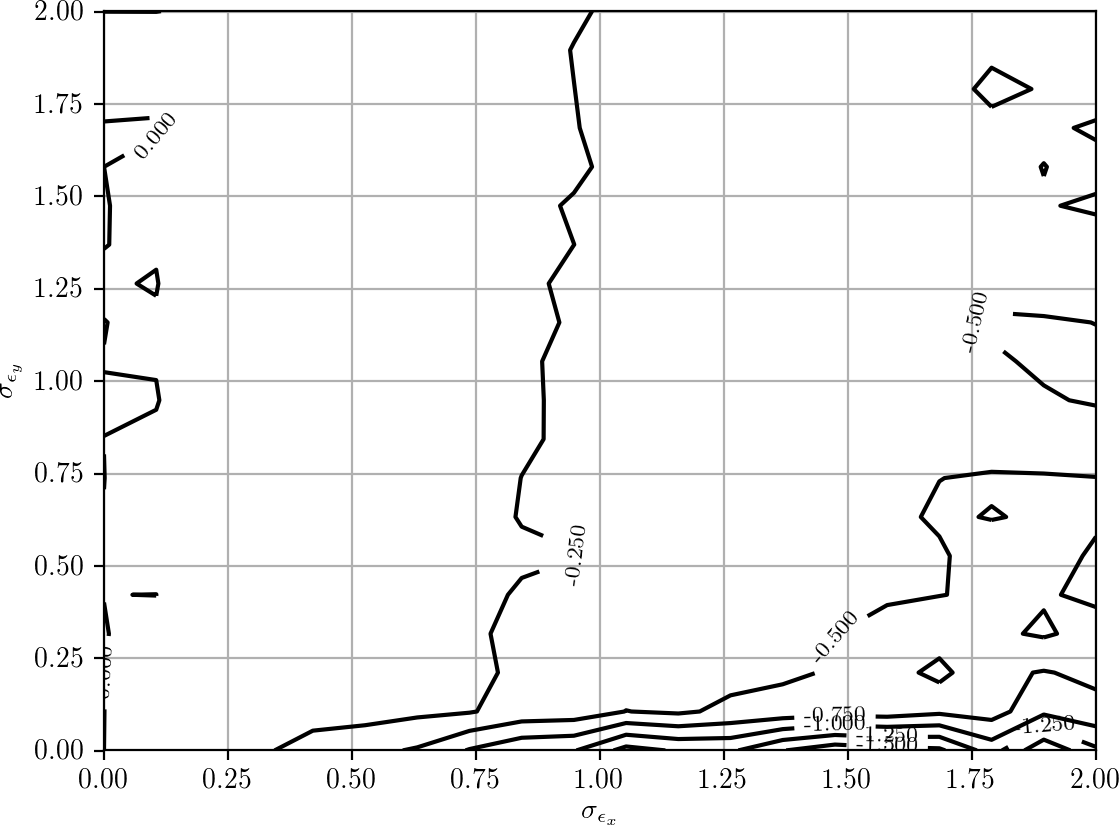
\includegraphics[width=135mm]{fig/nonlinear/linear/a-0_b-1.png}
  \caption{
    Сравнительная точность оценивания \\
    параметров линейной модели при \( \theta_1 = 1 \)
  }\label{fig:comparison_nonlinear_linear}
\end{figure}

\vspace{2\baselineskip}
\subsection{Параболическая функция регрессии}

Параболическая функция регрессии имеет следующий вид:
\[ \psi = \theta_0 + \theta_1 \xi + \theta_2 \xi^2. \]

На рисунках~\ref{fig:comparison_nonlinear_quadratic_b-0_c-1}--\ref{fig:comparison_nonlinear_quadratic_c-1} представлен ряд графиков зависимости
\( d(\sigma_{\varepsilon_x}, \sigma_{\varepsilon_y}) \)
для параболической функции регрессии при различных значениях её параметров.
По данным графикам можно сделать следующие выводы:
\begin{enumerate}
\item Точность оценивания параметров параболической модели не зависит
  от фактического значения постоянной составляющей \( \theta_0 \).
\item Если функция регрессии на промежутке аппроксимации является монотонной,
  то точность оценивания её параметров зависит главным образом от
  абсолютного значения её параметра \( \theta_2 \)
  (рисунок~\ref{fig:comparison_nonlinear_quadratic_b-5_c-1}).
  Чем большее абсолютное значение имеет данный параметр,
  тем более точными являются оценки, полученные НМНК,
  по сравнению с МРТ-оценками
  (рисунки~\ref{fig:comparison_nonlinear_quadratic_b-0_c-1},~\ref{fig:comparison_nonlinear_quadratic_b-0},~\ref{fig:comparison_nonlinear_quadratic_b-5_c-1}).
\item В случае, когда функция регрессии на промежутке аппроксимации является немонотонной,
  метод рядов Тейлора оценивает параметры модели более точно, чем НМНК
  (рисунок~\ref{fig:comparison_nonlinear_quadratic_b--5_c-1}).
\end{enumerate}

\begin{figure}[b]
  \centering
  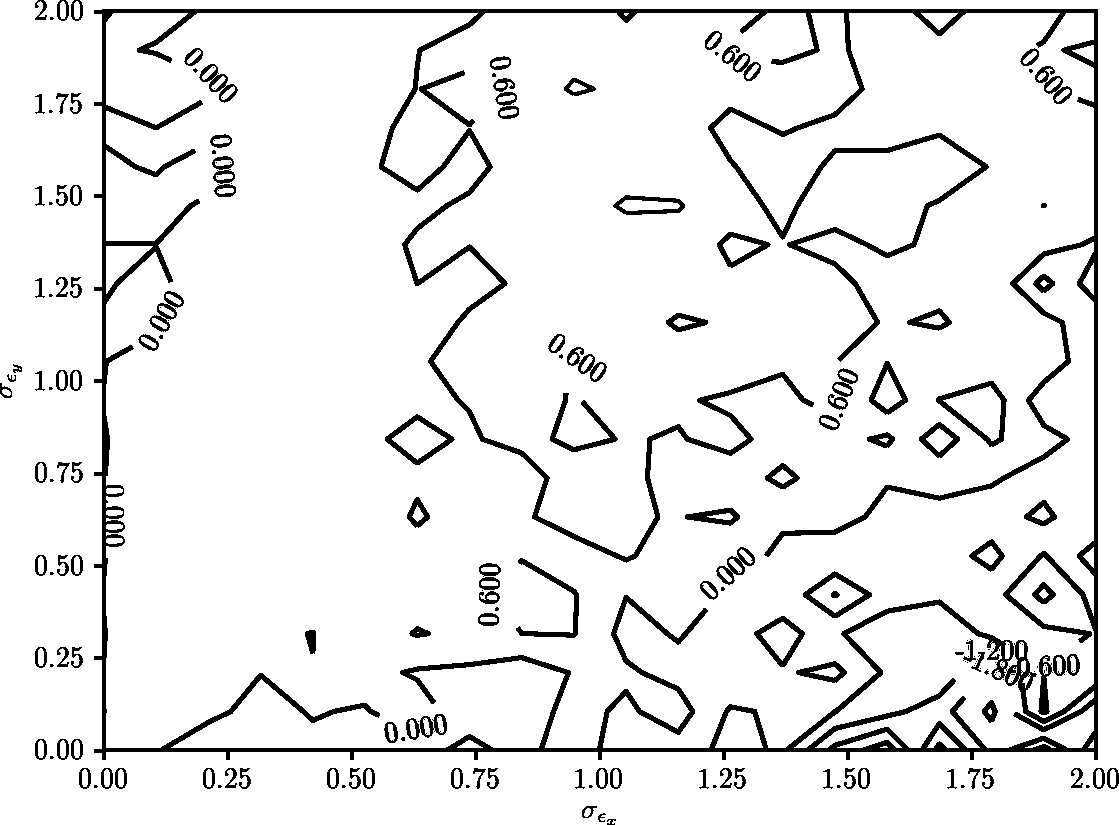
\includegraphics[width=135mm]{fig/nonlinear/quadratic/a-0_b-0_c-1.png}
  \caption{
    Сравнительная точность оценивания \\
    параметров параболической модели при \( \theta_1 = 0, \theta_2 = 1 \)
  }\label{fig:comparison_nonlinear_quadratic_b-0_c-1}
\end{figure}

\begin{figure}[p]
  \begin{subfigure}[b]{\linewidth}
    \centering
    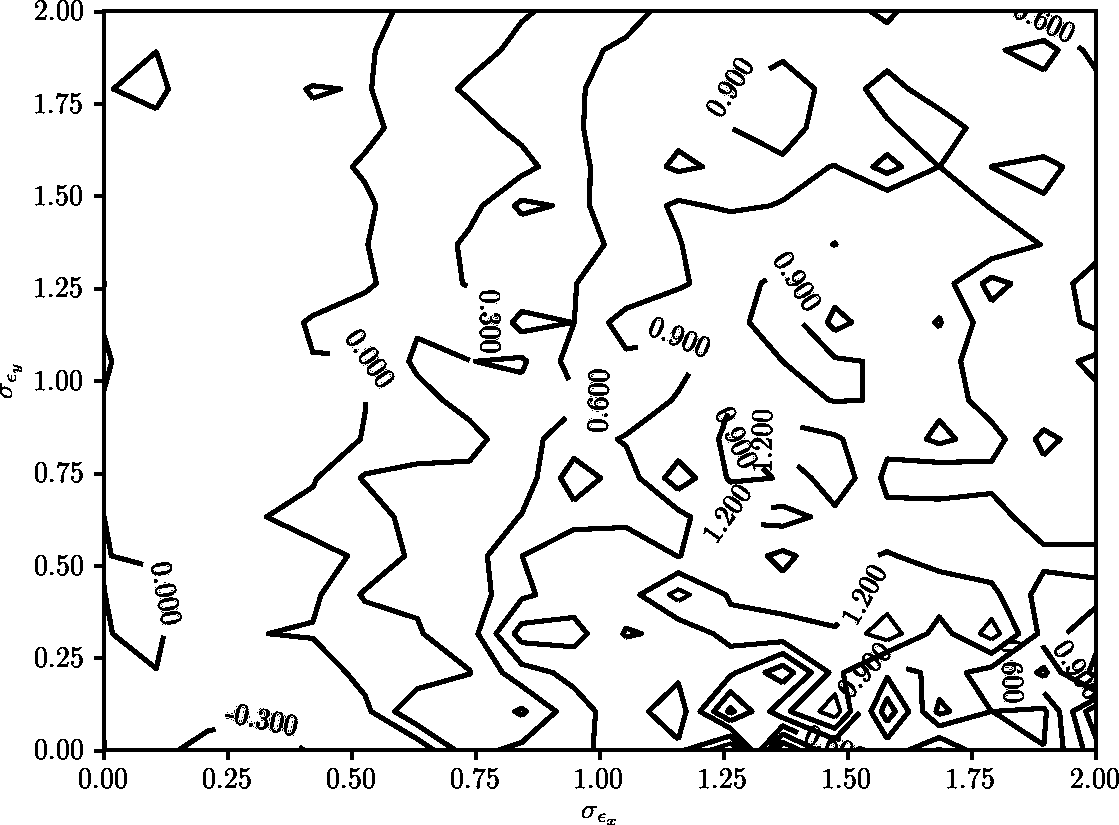
\includegraphics[width=135mm]{fig/nonlinear/quadratic/a-0_b--5_c-1.png}
    \caption{\( \theta_1 = -5 \)}\label{fig:comparison_nonlinear_quadratic_b--5_c-1}
  \end{subfigure}

  \vspace{2\baselineskip}
  \begin{subfigure}[b]{\linewidth}
    \centering
    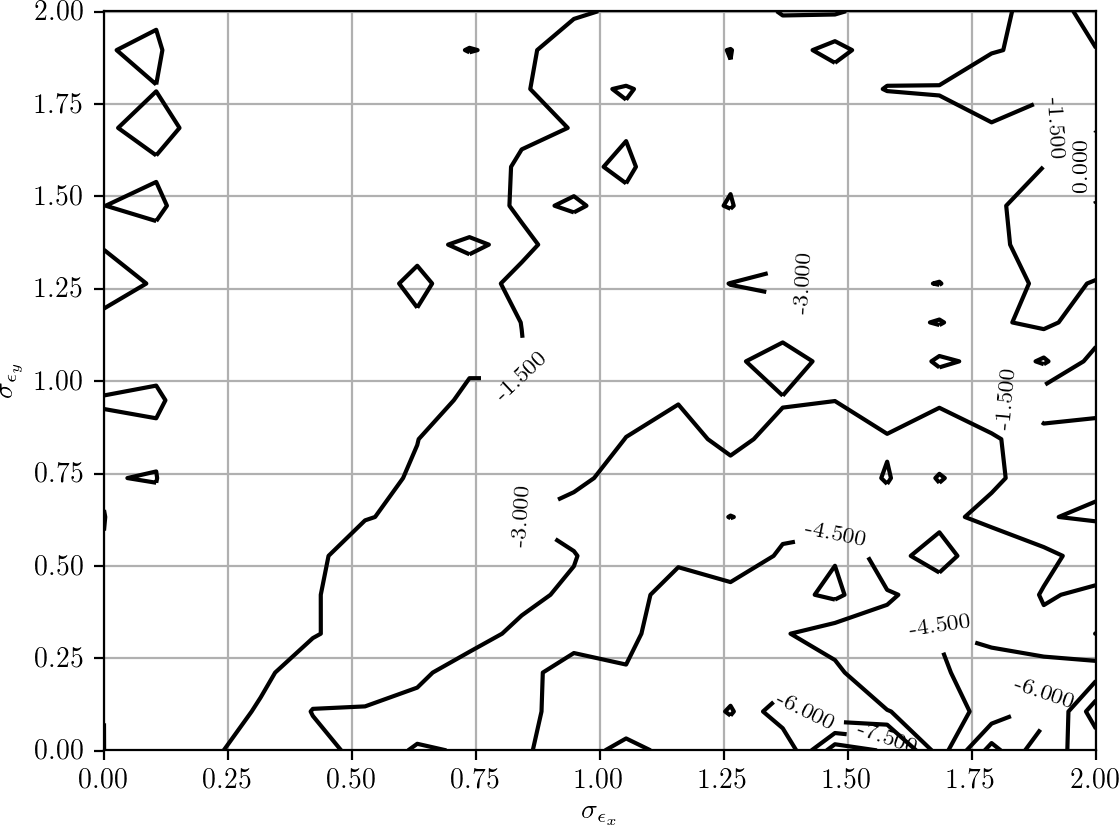
\includegraphics[width=135mm]{fig/nonlinear/quadratic/a-0_b-5_c-1.png}
    \caption{\( \theta_1 = 5 \)}\label{fig:comparison_nonlinear_quadratic_b-5_c-1}
  \end{subfigure}

  \vspace{\baselineskip}
  \caption{
    Сравнительная точность оценивания \\
    параметров параболической модели при \( \theta_2 = 1 \)
  }\label{fig:comparison_nonlinear_quadratic_c-1}
\end{figure}

\begin{figure}[p]
  \begin{subfigure}[b]{\linewidth}
    \centering
    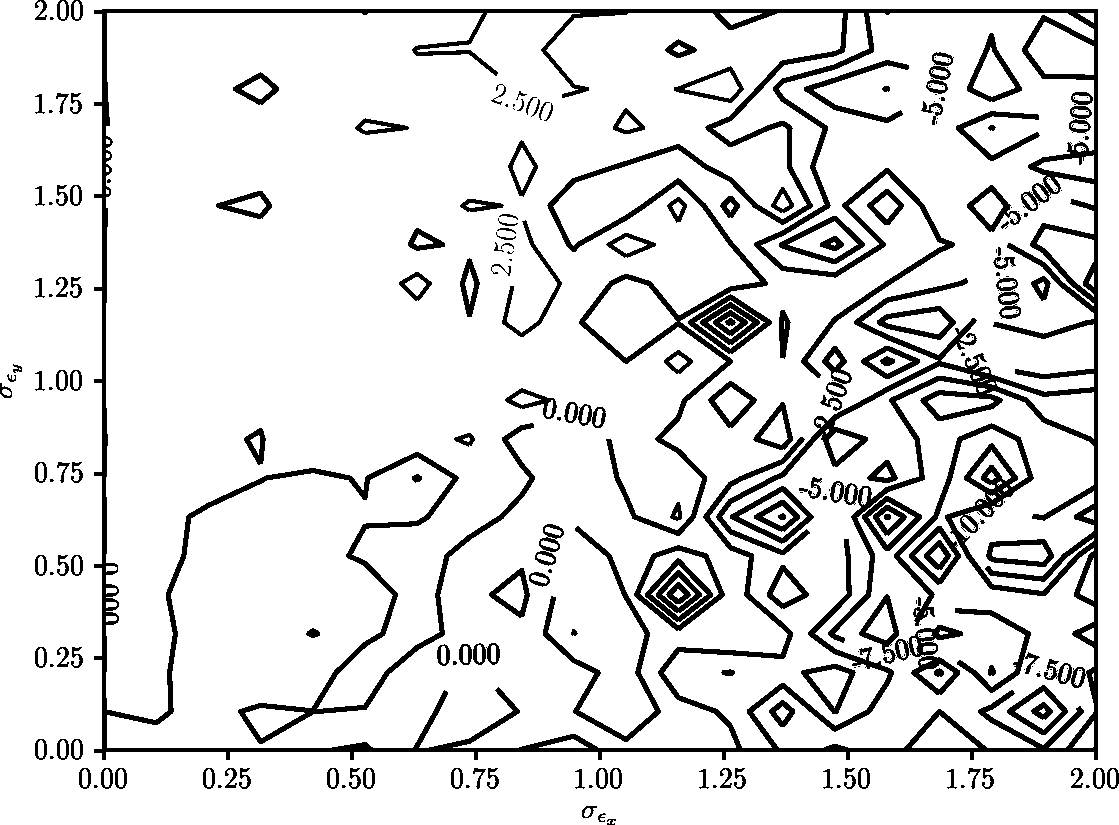
\includegraphics[width=135mm]{fig/nonlinear/quadratic/a-0_b-0_c--5.png}
    \caption{\( \theta_2 = -5 \)}
  \end{subfigure}

  \vspace{2\baselineskip}
  \begin{subfigure}[b]{\linewidth}
    \centering
    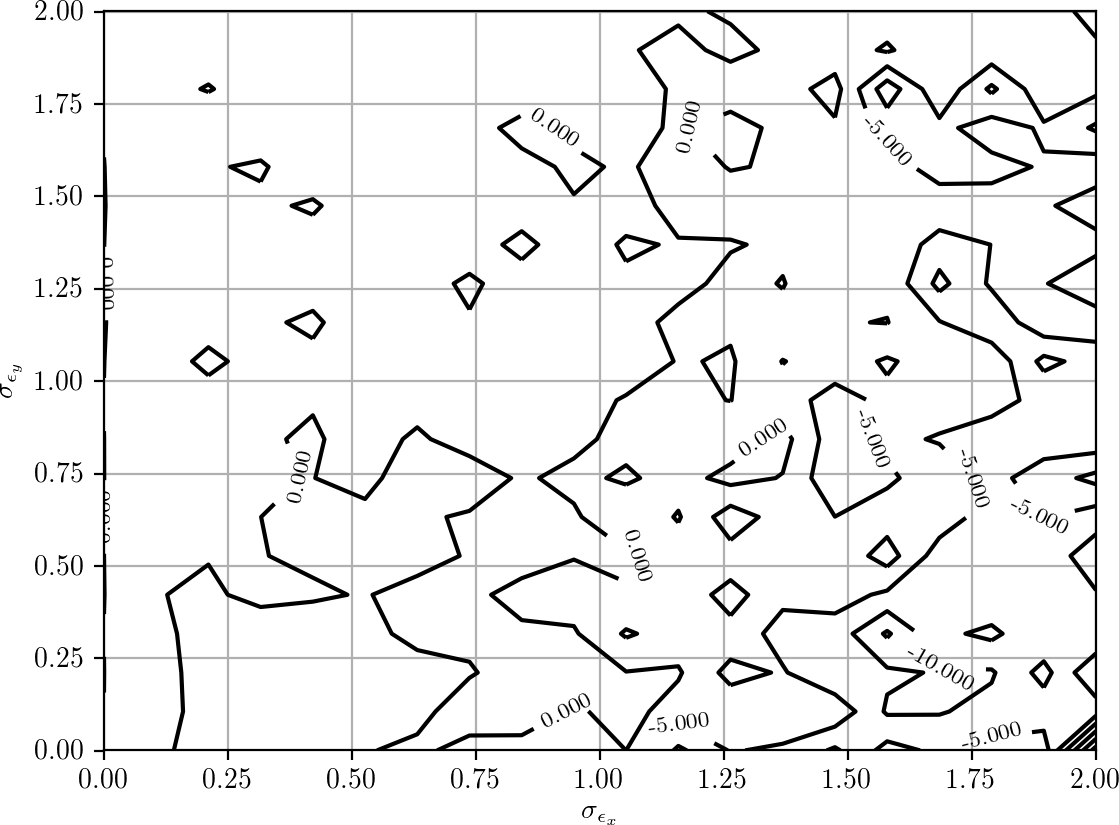
\includegraphics[width=135mm]{fig/nonlinear/quadratic/a-0_b-0_c-5.png}
    \caption{\( \theta_2 = 5 \)}
  \end{subfigure}

  \vspace{\baselineskip}
    \caption{
      Сравнительная точность оценивания \\
      параметров параболической модели при \( \theta_1 = 0 \)
    }\label{fig:comparison_nonlinear_quadratic_b-0}
\end{figure}

\vspace{2\baselineskip}
\subsection{Экспоненциальная функция регрессии}

Рассматривалась экспоненциальная функция регрессии вида
\[ \psi = e^{\theta_0 + \theta_1 \xi}, \; \theta_0 > 0, \theta_1 > 0. \]

На основании графиков зависимости \( d(\sigma_{\varepsilon_x}, \sigma_{\varepsilon_y}) \)
при различных значениях параметра \( \theta_1 \)
(рисунки~\ref{fig:comparison_nonlinear_exponential_a-2_b-0,3}--~\ref{fig:comparison_nonlinear_exponential_a-2_b-0,5}) можно сделать следующие выводы:
\begin{enumerate}
\item МРТ даёт в среднем более точные оценки параметров экспоненциальной модели, чем НМНК,
  во всем диапазоне рассматриваемых значений параметров \( \theta_0, \theta_1 \).
\item Чем большее значение имеют параметры модели \( \theta_0, \theta_1 \),
  тем более точными являются оценки, полученные МРТ, по сравнению с НМНК-оценками.
\end{enumerate}

\vspace{2\baselineskip}
\begin{figure}[h]
  \centering
  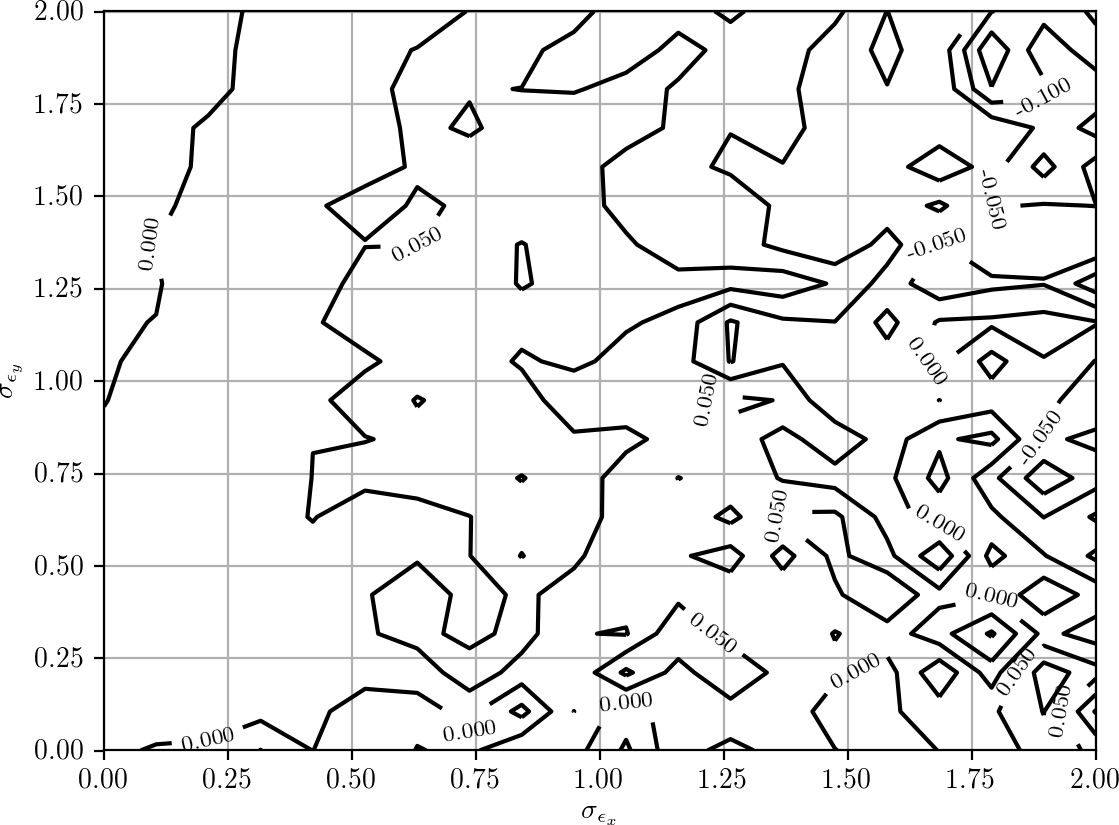
\includegraphics[width=135mm]{fig/nonlinear/exponential/a-2_b-0,3.png}
  \caption{
    Сравнительная точность оценивания \\
    параметров экспоненциальной модели при \( \theta_0 = 2, \theta_1 = 0{,}3 \)
  }\label{fig:comparison_nonlinear_exponential_a-2_b-0,3}
\end{figure}

\begin{figure}[p]
  \centering
  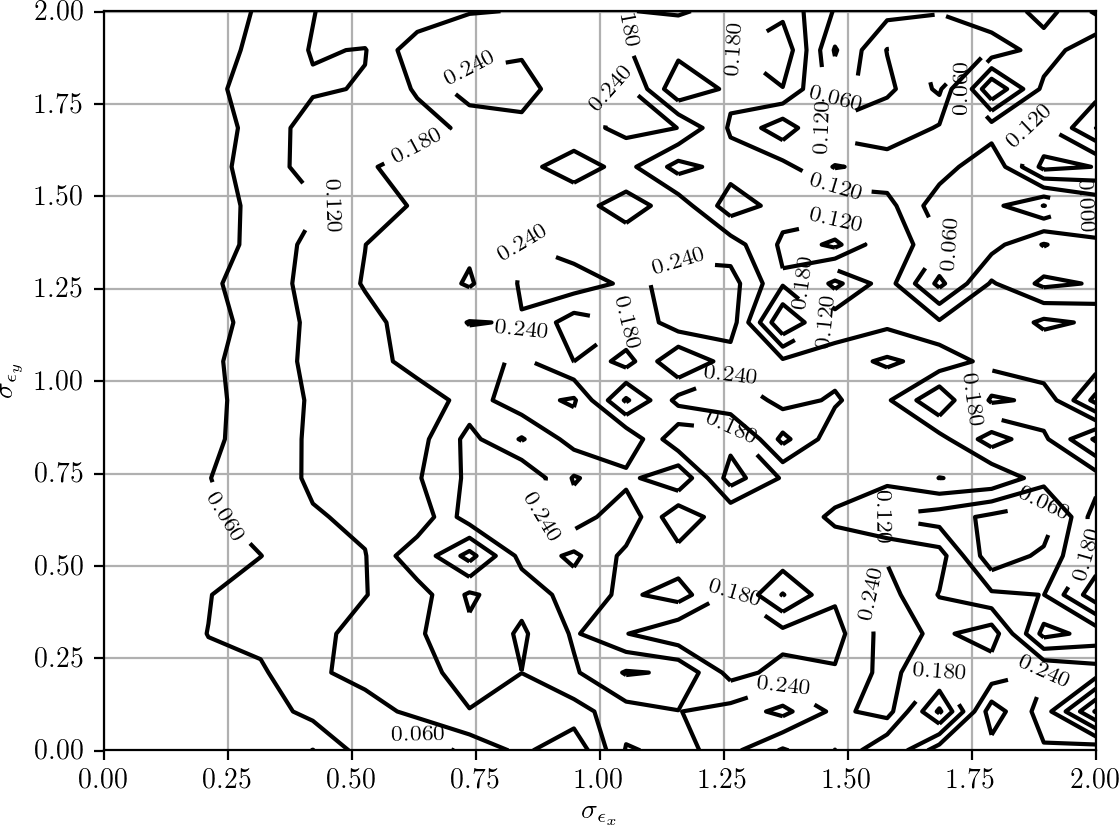
\includegraphics[width=135mm]{fig/nonlinear/exponential/a-2_b-0,4.png}
  \caption{
    Сравнительная точность оценивания \\
    параметров экспоненциальной модели при \( \theta_0 = 2, \theta_1 = 0{,}4 \)
  }\label{fig:comparison_nonlinear_exponential_a-2_b-0,4}
\end{figure}

\begin{figure}[p]
  \centering
  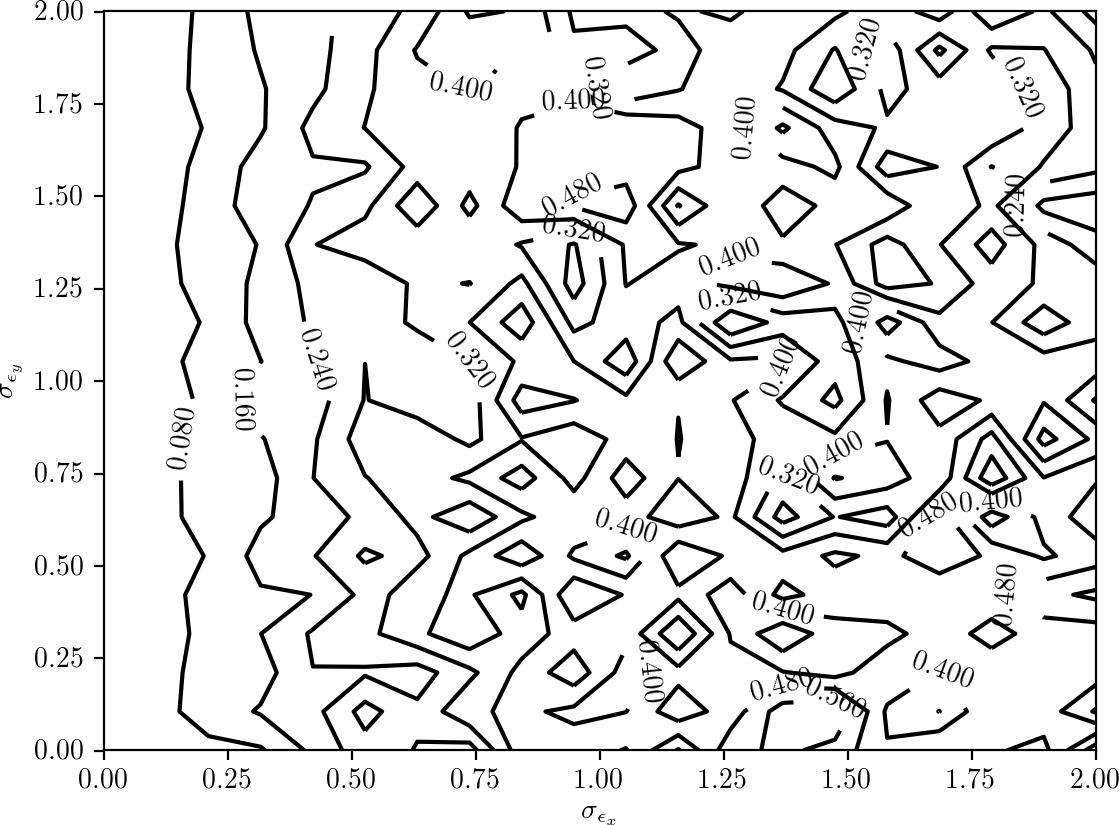
\includegraphics[width=135mm]{fig/nonlinear/exponential/a-2_b-0,5.png}
  \caption{
    Сравнительная точность оценивания \\
    параметров экспоненциальной модели при \( \theta_0 = 2, \theta_1 = 0{,}5 \)
  }\label{fig:comparison_nonlinear_exponential_a-2_b-0,5}
\end{figure}

\vspace{2\baselineskip}
\subsection{Обратная функция регрессии}

Под обратной функцией регрессии понимается выражение вида
\[ \psi = \theta_0 + \dfrac{1}{\theta_1 + \theta_2 x}. \]

Значения параметров \( \theta_1, \theta_2 \) выбирались таким образом, чтобы
их оценивание производилось по наблюдениям, соответствующим правой ветви функции \( \psi \).
В условиях моделирования, описанных в подразделе~\ref{subsec:nonlinear_comparison_conditions},
этого можно добиться, если принять
\[ c = \dfrac{\theta_1}{\theta_2} > 3 \max{(\sigma_{\varepsilon_x})} = 6. \]
Для того, чтобы исключить влияние горизонтального смещения функции регрессии,
необходимо, чтобы значение величины \( c \) сохранялось неизменным во всех экспериментах.

В таблице~\ref{tbl:comparison_nonlinear_inverse} приведены средние значения
величины \( d \) при различных значениях параметров \( \theta_1, \theta_2 \).
Нетрудно заметить, что во всех рассмотренных случаях средняя точность НМНК-оценок
является неудовлетворительной.
В этих же условиях МРТ даёт оценки приемлемой точности.

На рисунке~\ref{fig:comparison_nonlinear_inverse} представлены графики зависимости
\( d(\sigma_{\varepsilon_x}, \sigma_{\varepsilon_y}) \) при <<крайних>> значениях параметров
\( \theta_1, \theta_2 \), взятых из таблицы.
Видно, что при больших значениях ошибок с.~к.~о. наблюдений
МРТ позволяет получить значительно более точные оценки параметров, чем НМНК.
Данная тенденция проявляется тем сильнее,
чем менее пологой является функция регрессии при данных значениях параметров.
Кроме этого, следует отметить ряд пиковых значений на данных графиках,
сотвествующих случаям, когда опорные оценки параметров для НМНК были выбраны
особенно неудачно.

\begin{table}[b]
  \caption{%
    Средняя точность оценивания параметров обратной модели в
    зависимости от фактических значений параметров \( \theta_1, \theta_2 \)
  }\label{tbl:comparison_nonlinear_inverse}
  \small
  \begin{tabular}{| m{4cm} | M{3.7cm} | M{3.7cm} | M{3.7cm} |}
    \hline
    \( \theta_1, \theta_2 \)
    & \( avg(d_{\text{НМНК}}) \)
    & \( avg(d_{\text{МРТ}}) \)
    & \( avg(d_{\text{НМНК}} - d_{\text{МРТ}}) \) \\
    \hline
    \( \theta_1 = 0{,}035, \theta_2 = 0{,}005 \)
    & 1621{,}9
    & 14{,}8
    & 1607{,}1 \\
    \hline
    \( \theta_1 = 0{,}07, \theta_2 = 0{,}01 \)
    & 2533{,}9
    & 8
    & 2525{,}9 \\
    \hline
    \( \theta_1 = 0{,}14, \theta_2 = 0{,}02 \)
    & 2189
    & 4{,}3
    & 2184{,}7 \\
    \hline
    \( \theta_1 = 0{,}28, \theta_2 = 0{,}04 \)
    & 3358{,}1
    & 2{,}3
    & 3355{,}8 \\
    \hline
    \end{tabular}
\end{table}

\begin{figure}[p]
  \begin{subfigure}[b]{\linewidth}
    \centering
    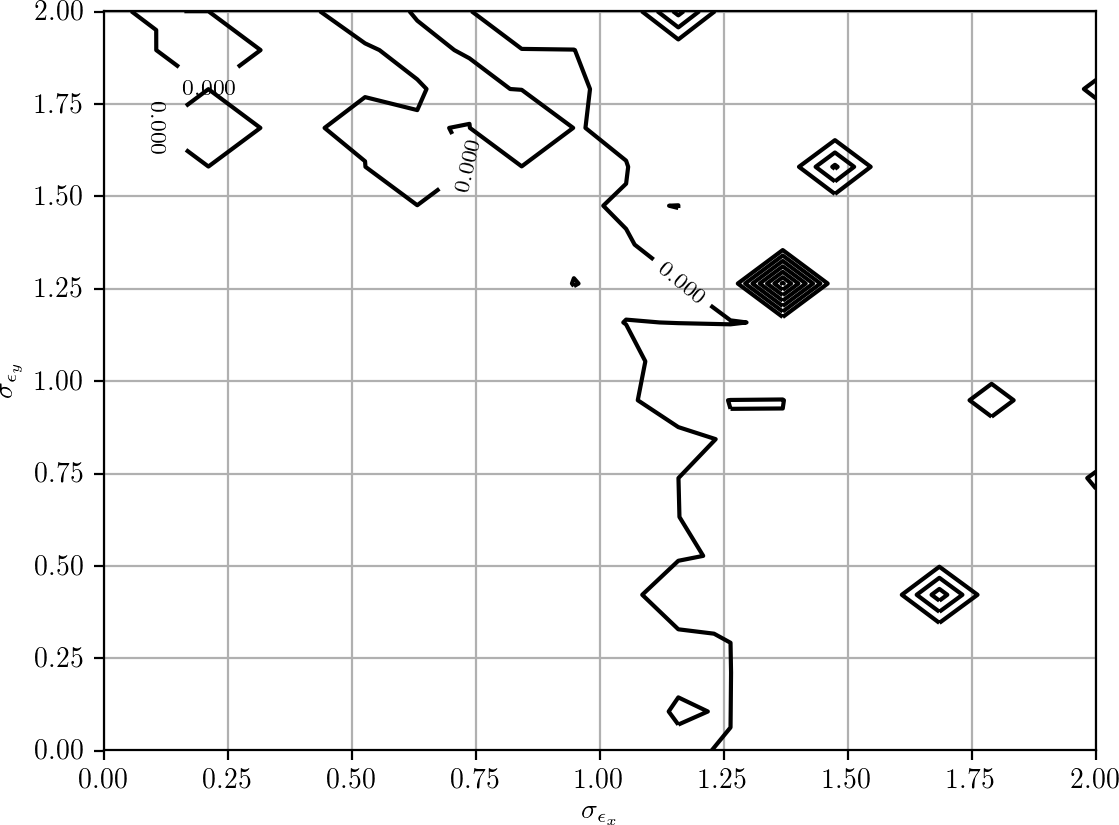
\includegraphics[width=135mm]{fig/nonlinear/inverse/a-0_b-0,035_c-0,005.png}
    \caption{\( \theta_1 = 0{,}035, \theta_2 = 0{,}05 \)}
  \end{subfigure}

  \vspace{2\baselineskip}
  \begin{subfigure}[b]{\linewidth}
    \centering
    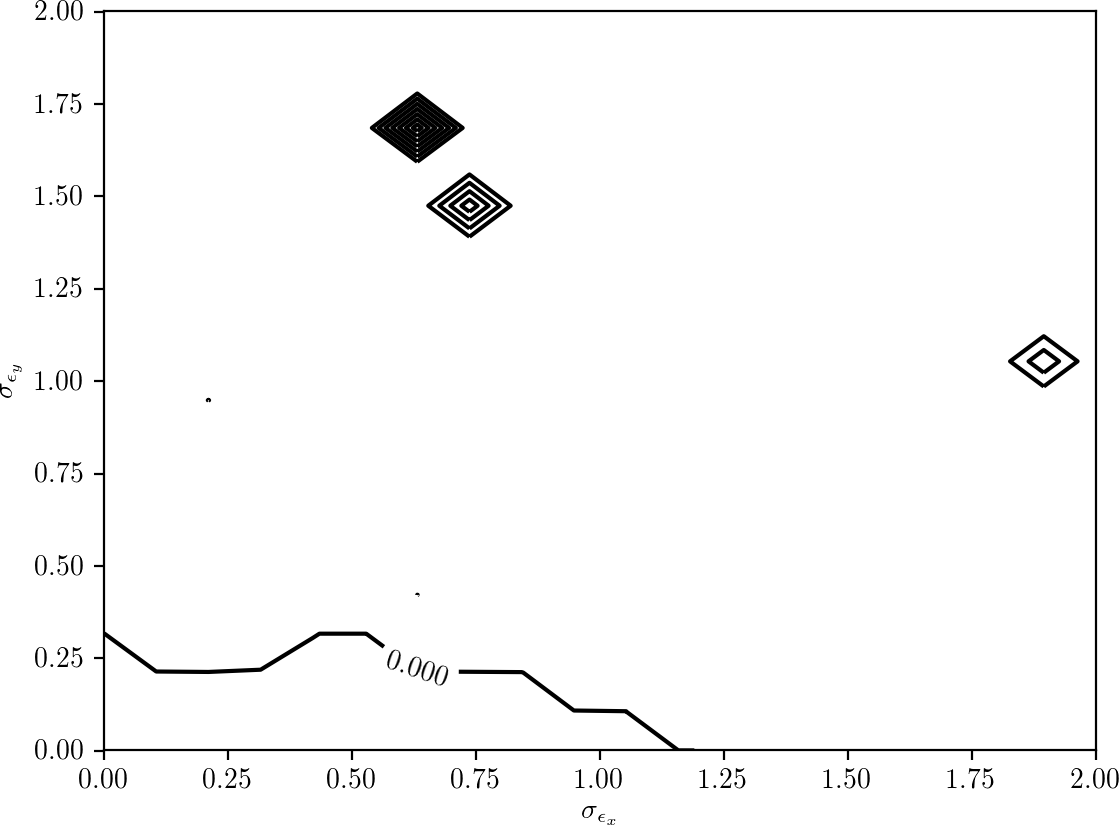
\includegraphics[width=135mm]{fig/nonlinear/inverse/a-0_b-0,28_c-0,04.png}
    \caption{\( \theta_1 = 0{,}28, \theta_2 = 0{,}4 \)}
  \end{subfigure}

  \vspace{\baselineskip}
    \caption{
      Сравнительная точность оценивания \\
      параметров обратной модели
    }\label{fig:comparison_nonlinear_inverse}
\end{figure}

\vspace{2\baselineskip}
\subsection{Синусоидальная функция регрессии}

Рассматривалось семейство функций регрессии вида
\[ \psi_{\varphi} = \theta_0 + \theta_1 \sin{(\varphi \xi)}, \:
\varphi \in \{ 0{,}2, 1, 5 \}. \]

В таблице~\ref{tbl:comparison_nonlinear_sinusoidal} приведены средние значения
величин \( d \) при различных значениях параметров \( \theta_1 \).
По данным таблицы можно сделать вывод, что в среднем НМНК оценивает параметры
синусоидальных функций регрессии точнее, чем МРТ.
Сравнительная точность оценивания зависит как от частоты \( \varphi \)
(нелинейным образом), так и от коэффициента усиления
(с ростом \( \theta_1 \) точность НМНК-оценивания снижается медленнее, чем МРТ).

На рисунке~\ref{fig:comparison_nonlinear_sinusoidal}
представлены графики функции \( d(\sigma_{\varepsilon_x}, \sigma_{\varepsilon_y}) \)
для синусоидальной функции регрессии \( \psi_{1} \) при
различных значениях параметра \( \theta_1 \).
Видно, что точность оценок, полученных с помощью НМНК, оказывается выше,
чем МРТ-оценок, при любых значениях с.~к.~о. ошибок измерений.
Данная тенденция проявляется наиболее сильно при
\( \sigma_{\varepsilon_x} \gg \sigma_{\varepsilon_y} \),
что вызвано, по-видимому, тем фактом, что синусоидальная функция
является периодической.

\begin{table}[h]
  \caption{%
    Средняя точность оценивания параметров синусоидальной модели в
    зависимости от частоты \( \varphi \) и фактических значений параметра \( \theta_1 \)
  }\label{tbl:comparison_nonlinear_sinusoidal}
  \begin{tabular}{| M{1.3cm} | M{1.3cm} | M{4cm} | M{4cm} | M{4cm} |}
    \hline
    \( \varphi \)
    & \( \theta_1 \)
    & \( avg(d_{\text{НМНК}}) \)
    & \( avg(d_{\text{МРТ}}) \)
    & \( avg(d_{\text{НМНК}} - d_{\text{МРТ}}) \) \\
    \hline
    \multirow{3}{*}{0{,}5}
    & 2
    & 0{,}36
    & 0{,}45
    & -0{,}09 \\ \cline{2-5}
    & 5
    & 0{,}78
    & 1{,}03
    & -0{,}25 \\ \cline{2-5}
    & 10
    & 1{,}51
    & 2{,}03
    & -0{,}52 \\
    \hline
    \multirow{3}{*}{1}
    & 2
    & 0{,}93
    & 1{,}06
    & -0{,}12 \\ \cline{2-5}
    & 5
    & 2{,}27
    & 2{,}64
    & -0{,}37 \\ \cline{2-5}
    & 10
    & 4{,}51
    & 5{,}39
    & -0{,}87 \\
    \hline
    \multirow{3}{*}{2}
    & 2
    & 1{,}39
    & 1{,}47
    & -0{,}08 \\ \cline{2-5}
    & 5
    & 3{,}44
    & 3{,}67
    & -0{,}23 \\ \cline{2-5}
    & 10
    & 6{,}86
    & 7{,}44
    & -0{,}57 \\
    \hline
    \end{tabular}
\end{table}

% Во всех описанных случаях оценивания параметров
% НМНК-оценки являются более точными.
% Следует отметить, что при малых ошибках измерений выходной переменной
% нелинейный метод наименьших квадратов дает значительно более точные оценки.


\begin{figure}[p]
  \begin{subfigure}[b]{\linewidth}
    \centering
    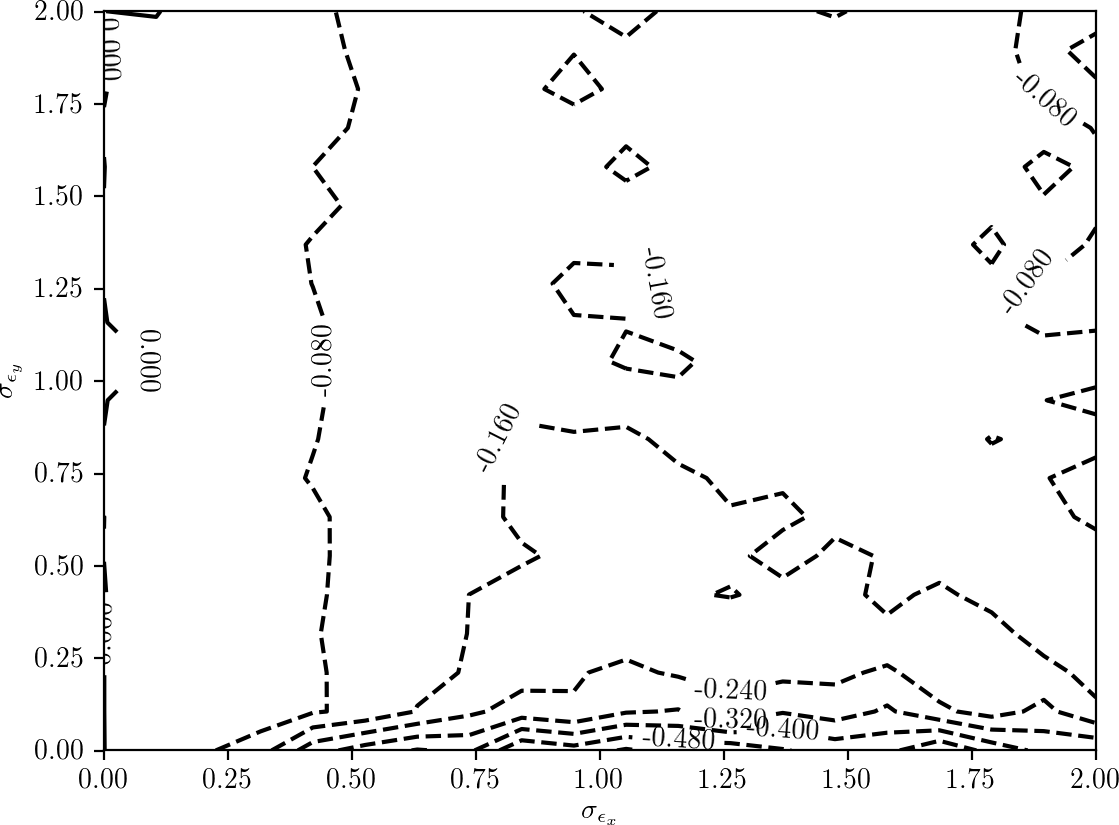
\includegraphics[width=135mm]{fig/nonlinear/sinusoidal/a-0_b-2.png}
    \caption{\( \theta_1 = 2 \)}
  \end{subfigure}

  \vspace{2\baselineskip}
  \begin{subfigure}[b]{\linewidth}
    \centering
    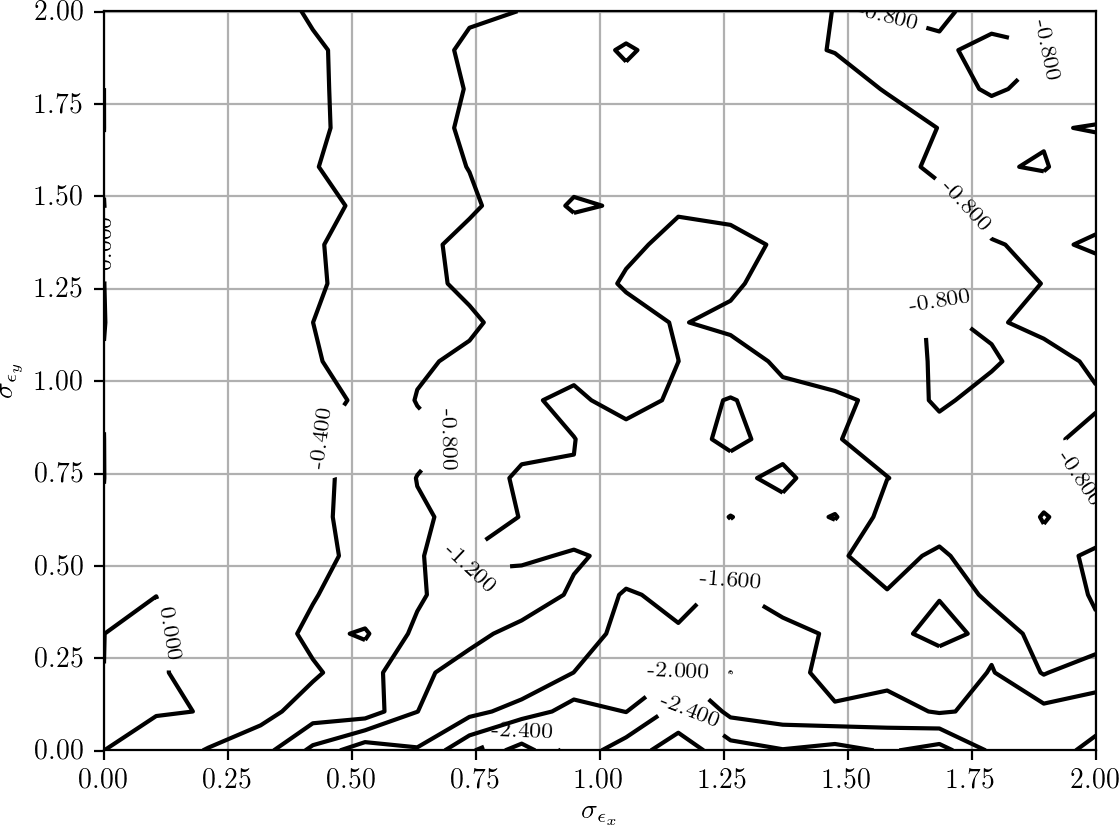
\includegraphics[width=135mm]{fig/nonlinear/sinusoidal/a-0_b-10.png}
    \caption{\( \theta_1 = 5 \)}
  \end{subfigure}

  \vspace{\baselineskip}
  \caption{
    Сравнительная точность оценивания \\
    параметров синусоидальной модели
  }\label{fig:comparison_nonlinear_sinusoidal}
\end{figure}


% Рассматривались функции регрессии вида
% \begin{equation*}
%   \psi = \theta_0 + \dfrac{1}{\theta_1 + \theta_2 \xi}.
% \end{equation*}

% На рисунках~\ref{fig:comparison_nonlinear_hyperbolic_a-0_b-0,001}--\ref{fig:comparison_nonlinear_hyperbolic_a-0_b-1}
% представлены графики функции \( d(\sigma_{\varepsilon_x}, \sigma_{\varepsilon_y}) \)
% для обратной функции регрессии \( \psi \) при
% различных значениях параметра \( \theta_2 \).
% {\color{red}Во всех описанных случаях оценивания параметров
% МРТ-оценки являются более точными.
% Кроме этого, отдельные оценки, полученные НМНК,
% являются совершенно неудовлетворительными,
% о чем свидетельствуют "пики" на приведенных графиках.
% }

% \begin{figure}[h]
%   \centering
%   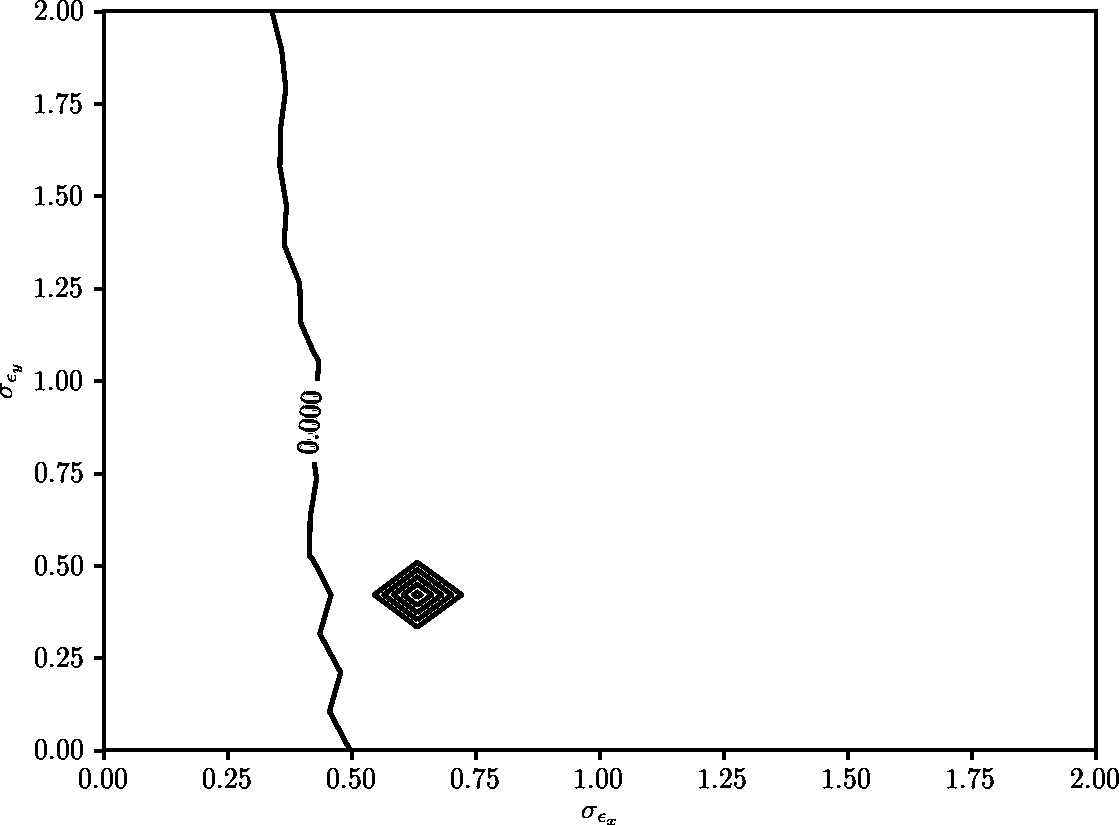
\includegraphics[width=135mm]{fig/nonlinear/hyperbolic/a-0_b-0,001.png}
%   \caption{
%     Точность оценивания параметров \\
%     гиперболической модели при \( \theta_1 = 0,001 \)
%   }\label{fig:comparison_nonlinear_hyperbolic_a-0_b-0,001}
% \end{figure}

% \begin{figure}[h]
%   \centering
%   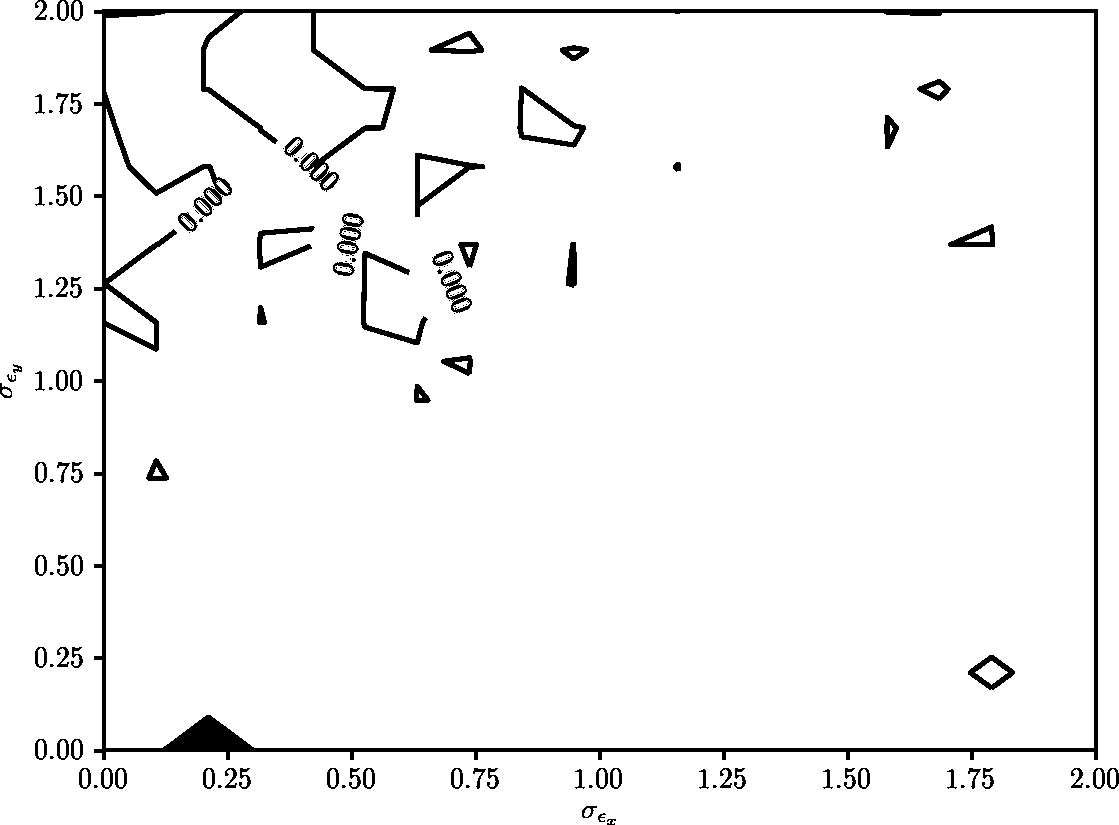
\includegraphics[width=135mm]{fig/nonlinear/hyperbolic/a-0_b-1.png}
%   \caption{
%     Точность оценивания параметров \\
%     гиперболической модели при \( \theta_1 = 1 \)
%   }\label{fig:comparison_nonlinear_hyperbolic_a-0_b-1}
% \end{figure}


% % \subsection{Экспоненциальная функция регрессии}
% % гиперболическая функция регрессии
% % степенная и показательная функции

% % \subsection{Степенная функция регрессии}

% % Рассматривались функции регрессии вида
% % \begin{equation*}
% %   \psi = \theta_1 \xi^{\theta_2}.
% % \end{equation*}


% % нелинейным регрессиям по оцениваемым параметрам
% \subsection{Синусоидальная функция регрессии}

% Рассматривались функции регрессии вида
% \begin{equation*}
%   \begin{aligned}
%     \psi_1 &= \theta_0 + \theta_1 \sin{0{,}2 \xi}, \\
%     \psi_2 &= \theta_0 + \theta_1 \sin{\xi}, \\
%     \psi_3 &= \theta_0 + \theta_1 \sin{5 \xi}.
%   \end{aligned}
% \end{equation*}

% На рисунках~\ref{fig:comparison_nonlinear_sinusoidal}
% представлены графики функции \( d(\sigma_{\varepsilon_x}, \sigma_{\varepsilon_y}) \)
% для синусоидальной функции регрессии \( \psi_2 \) при
% различных значениях параметра \( \theta_1 \).
% Во всех описанных случаях оценивания параметров
% НМНК-оценки являются более точными.
% Следует отметить, что при малых ошибках измерений выходной переменной
% нелинейный метод наименьших квадратов дает значительно более точные оценки.

% \begin{figure}[b]
%   \begin{subfigure}[b]{\linewidth}
%     \centering
%     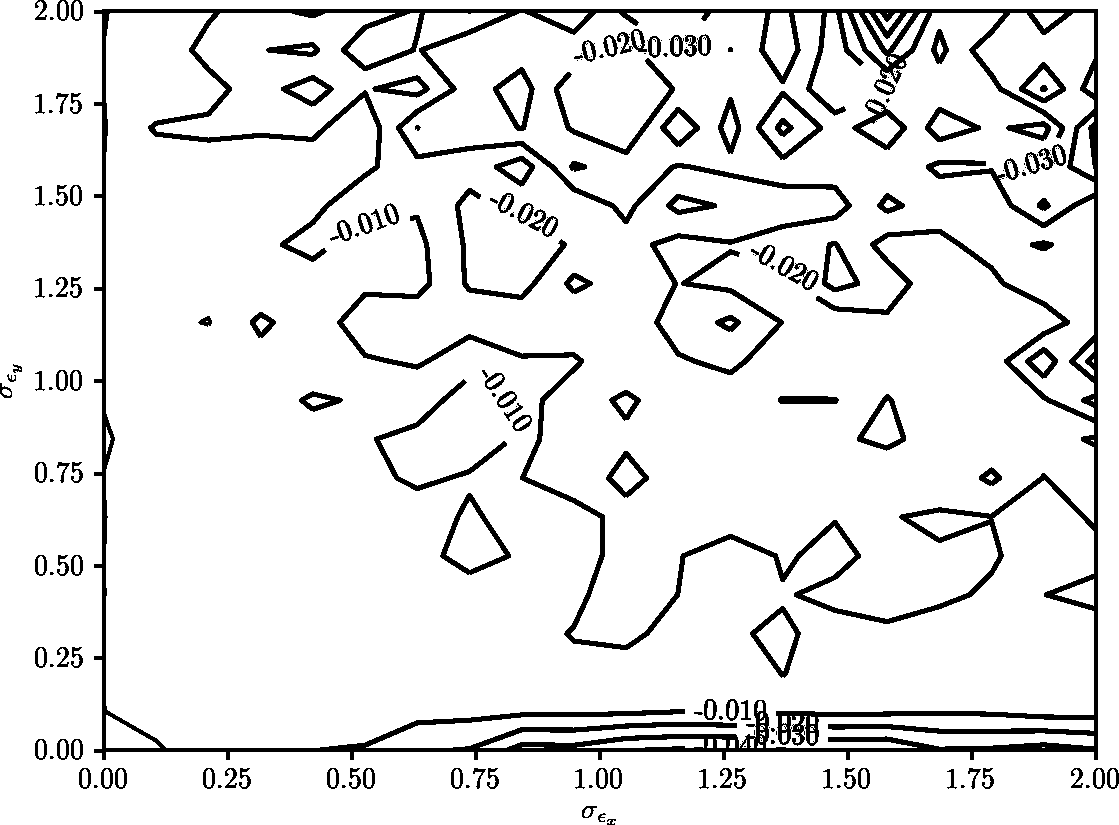
\includegraphics[width=135mm]{fig/nonlinear/sinusoidal/a-0_b-0,2.png}
%     \caption{\( \theta_1 = 0,2 \)}
%   \end{subfigure}

%   \vspace{2\baselineskip}
%   \begin{subfigure}[b]{\linewidth}
%   \centering
%   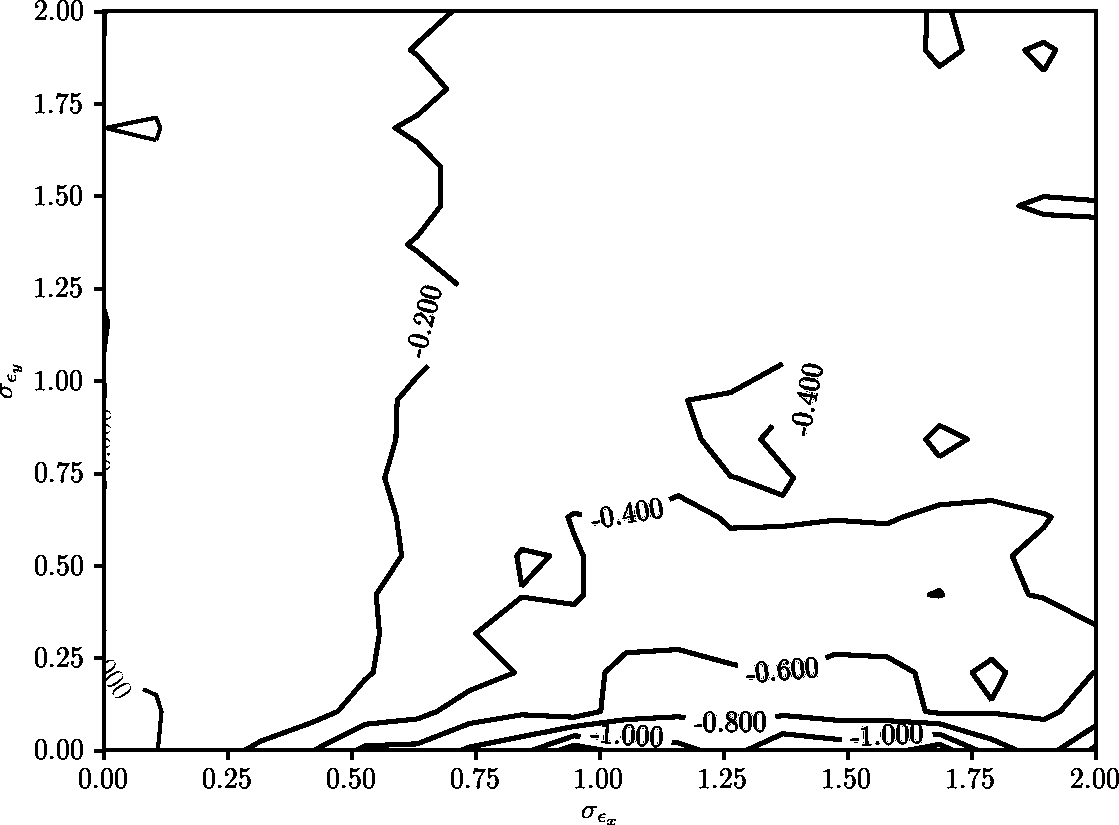
\includegraphics[width=135mm]{fig/nonlinear/sinusoidal/a-0_b-5.png}
%   \caption{\( \theta_1 = 5 \)}
% \end{subfigure}

% \vspace{\baselineskip}
%   \caption{
%     Точность оценивания параметров \\
%     синусоидальной модели
%   }\label{fig:comparison_nonlinear_sinusoidal}
% \end{figure}

%
% Точность НМНК существенным образом зависит от того, насколько удачной оказалась опорная оценка.
% В некоторых случаях получить хорошую опорную оценку проблематично.
% МРТ не зависит от опорных оценок и дает хорошие результаты там, где НМНК дает осечку.
% Предлагается использовать МРТ-оценку в качестве опорной для НМНК.
%

% \begin{table}[h!]
%   \caption{%
%     Средняя точность оценивания параметров экспоненциальной модели в
%     зависимости от фактических значений параметра \( \theta_1 \)
%   }
%   \small
%   \begin{tabular}{| m{3.75cm} | m{3.75cm} | m{3.75cm} | m{3.75cm} |}
%     \hline
%     \( \theta_1 \)
%     & \( avg(d_{\text{НМНК}}) \)
%     & \( avg(d_{\text{МРТ}}) \)
%     & \( avg(d_{\text{НМНК}} - d_{\text{МРТ}}) \) \\
%     \hline
%     0{,}3
%     &
%     &
%     & \\
%     \hline
%     0{,}4
%     &
%     &
%     & \\
%     \hline
%     0{,}5
%     &
%     &
%     & \\
%     \hline
%     \end{tabular}
% \end{table}
